% !TeX program = lualatex
% !TeX encoding = utf8
% !TeX spellcheck = uk_UA
% !BIB program = bibtex8

\documentclass{LabWork}
\graphicspath{{LabWork5pic/}}
\usetikzlibrary{arrows.meta}
\tikzset{
every info/.style={font=\small},
}
\usetikzlibrary{decorations.pathreplacing}

%============================================= Заголовок документу ====================================================%
\work{5}
\title{Вимірювання величини електричного опору за допомогою містка Уітстона}

%\author{}{}

%\group{ФФ-93}

\abstract{%

Вивчення принципу роботи вимірювальної мостової схеми. Визначення величини опору двох провідників і величини опору при їх послідовному і паралельному з'єднанні. Визначення величини внутрішнього опору гальванометра.
}
%======================================================================================================================%

\begin{document}
\writedatatofile{\jobname}
\maketitle

\section{Теоретичні відомості}

\begin{wrapfigure}{O}{0.3\linewidth}\centering
	\begin{tikzpicture}[thick, every circuit symbol/.style={thick},large circuit symbols,
			current/.style={black, font=\small, inner sep = 2pt},
		]
		\node (A) [contact] at (0,4) {}; \node [left]  at (A) {$A$};
		\node (B) [contact] at (4,4) {}; \node [right] at (B) {$B$};
		\node (C) [contact] at (2,6) {}; \node [above] at (C) {$C$};
		\node (D) [contact] at (2,2) {}; \node [below] at (D) {$D$};
		\draw (A)  -- (0,0) to[battery={info=$\mathcal{E}$}] (4,0) -- (B) ;
		\draw (A)  to[resistor={info=$R_1$}]  (C)
		(C)  to[resistor={info=$R_2$}]  (B)
		(B)  to[resistor={info=$R_3$}]  (D)
		(D)  to[resistor={info=$R_4$}]  (A);
		\draw (D) to [resistor={info=$R_e$, fill=red!40}]  (C);
		\draw[-latex, red, thick, shift={(0pt,0pt)}, font=\small] (0,0) --  node[right, black] {$I$} ++(0,1);
		\draw[-latex, red, thick] (A) --  node[anchor={south east}, current] {$I_1$} ++(45:0.75);
		\draw[-latex, red, thick] (C) --  node[anchor={south west}, current] {$I_2$} ++(-45:0.75);
		\draw[-latex, red, thick] (D) --   node[anchor={north west}, current] {$I_3$}++(45:0.75) ;
		\draw[-latex, red, thick] (A) --   ++(-45:0.75) node[anchor={north east}, current] {$I_4$};
		\draw[-latex, red, thick, shift={(0pt,0pt)}] (C) --  node[anchor={north west}, current] {$I_e$}  ++(0,-0.75) ;
	\end{tikzpicture}
	\caption{Місток Уітсона}
	\label{picBridge}
\end{wrapfigure}
Містком Уітсона в техніці вимірювань називають електричний прилад для вимірювання опорів, ємностей, індуктивностей та інших електричних величин, що представляють собою вимірювальну мостове коло, дія якого базується на методиці порівняння вимірюваної величини з зразковою мірою. Як відомо, метод порівняння дає досить точні результати вимірювань, внаслідок чого мостові схеми набули широкого поширення як в лабораторній, так і у виробничій практиці.

Класичне мостове коло складається з чотирьох опорів $R_1$, $R_2$, $R_3$ та $R_4$, які з'єднані послідовно у вигляді чотирикутника (рис.~\ref{picBridge}), причому точки $A$, $B$, $C$, $D$ називають \emph{вершинами}. Гілка $AB$, що містить джерело живлення $\mathcal{E}$, називається \emph{діагоналлю живлення}, а гілка $CD$, що містить опір навантаження $R_e$~--- \emph{діагоналлю навантаження}. Гілки $AC$, $CB$, $BC$ та $DA$, які містять опори $R_1$, $R_2$, $R_3$ та $R_4$ називаються \emph{плечима містка}.


Міст можна привести в стан рівноваги, який настає, коли потенціали вершин $C$ та $D$ стануть однаковими $\phi_C = \phi_D$. В цьому випадку струм через ділянку не йтиме $I_e = 0$. Така ситуація, як можна показати на основі законів Ома, можлива при рівності напруг на плечах $AC$ і $AD$ та на плечах $CB$ і $BD$, тобто тобто при $I_1R_1 = I_4R_4$ і $I_2R_2 = I_3R_3$. 

\begin{More}
    Дійсно, з законів Ома випливає що для плечей $AC$ і $AD$:
    \begin{equation}\label{}
        \begin{cases}
            \phi_A - \phi_C = I_1R_1, \\
            \phi_A - \phi_D = I_4R_4.
        \end{cases}
    \end{equation} 
І віднявши перше рівняння системи від другого, матимемо:
    \begin{equation}\label{}
        \phi_D - \phi_C = I_1R_1 - I_4R_4.
    \end{equation}
Для умови рівноваги містка повинно бути $\phi_D - \phi_С = 0$, а тому $I_1R_1 = I_4R_4$. Аналогічні міркування для плечей $CB$ і $BD$ дають умову $I_2R_2 = I_3R_3$.
\end{More}

А оскільки $I_e = 0$, то $I_1 = I_2$ та $I_3 = I_4$ (струм у вузлах не розгалужується), тому умову рівноваги можна записати у вигляді:
\begin{equation}\label{BridgeEquality}
	\frac{R_1}{R_2} = \frac{R_4}{R_3}.
\end{equation}

Рівновагу містка буде порушено, якщо в будь-якому плечі зміниться опір. Тоді зміняться струми в гілках, зміняться потенціали вузлів $C$ і $D$ ($\phi_C \neq \phi_D$). В діагоналі $CD$ з'явиться струм. Такий місток називається \emph{неврівноваженим}.

\subsection{Принцип вимірювання опору містком}

Для вимірювання опору містком необхідно, щоб одне плече мало опір відомої величини $R$, а інше~--- опір невідомої величини $R_x$, який, власне, і треба виміряти. В двох інших плечах опори можна підбирати за допомогою \emph{реохорда} (рис.~\ref{MeasurBridge}).

\begin{wrapfigure}{O}{0.5\linewidth}\centering
	\begin{tikzpicture}[thick, every circuit symbol/.style={thick},large circuit symbols,
			current/.style={black, font=\small, inner sep = 2pt},
		]
		\node (A) [contact] at (0,2) {}; \node [left]  at (A) {$A$};
		\node (B) [contact] at (6,2) {}; \node [right] at (B) {$B$};
		\node (C) [contact] at (3,6) {}; \node [above] at (C) {$C$};
		%                    \node (D) [contact] at (2,2) {}; \node [below] at (D) {$D$};
		\draw[thick] (A) -- coordinate[pos=0.4] (D) (B);
		\draw (A)  -- (0,0) to[battery={info=$\mathcal{E}$}] ++(3,0) to[make contact] ++(3,0) -- (B) ;
		\draw (A)  to[resistor={info=$R_x$, fill=cyan!50}] (C) ;
		\draw (C)  to[resistor={info=$R$}] (B) ;
		\draw (C) to[galvanometer] ++(0,-2.5) coordinate (G);
		\draw[-latex] (G) .. controls (3,2) and (2.5,4) .. (D) node[below=5pt] {$D$};
		\draw[decoration={brace,mirror,raise=1pt, amplitude=5pt},decorate,red] (A) -- (D) node[midway, below=5pt, current] {$l_1$};
		\draw[decoration={brace,mirror,raise=1pt, amplitude=5pt},decorate, red] (D) -- (B) node[midway, below=5pt, current] {$l_2$};
	\end{tikzpicture}
	\caption{Принцип вимірювання опору}
	\label{MeasurBridge}
\end{wrapfigure}
Реохорд (ділянка $AB$ на рис.~\ref{MeasurBridge})  являє собою однорідний дріт з високим опором, який укріплений на лінійці уздовж якої може переміщуватися ковзний контакт $D$. Переміщуючи ковзний контакт $D$  вздовж дроту  можна неперервним чином змінювати опори плечей $AD$: $R_{AD} = \rho\frac{l_1}{S}$ та $DB$: $R_{DB} = \rho\frac{l_2}{S}$, які залежать від довжин цих плечей $l_1$ та $l_2$, відповідно. Рухаючи повзунок, можна домогтись рівноваги містка, що фіксується нульовими показами гальванометра $G$ (струм через гальванометр не тече). Використовуючи умову рівноваги~\eqref{BridgeEquality} для випаду міст\-ка з реохордом, можна знайти величину шуканого опору:
\begin{equation}\label{BridgeEqualityRheo}
	R_x = R \frac{l_1}{l_2}.
\end{equation}

\section{Точність вимірювання опору за допомогою містка Уітстона}

Визначимо, від чого залежить точність вимірювання методом містка Уітстона. Для цього зробимо деякі спрощення. Так як сумарна довжина реохорда $L = l_1 + l_2$, то  \eqref{BridgeEqualityRheo} виразивши $l_2$, можна записати у вигляді
\begin{equation}\label{BridgeEqualityRheo2}
	R_x = R \frac{l_1}{L - l_1}.
\end{equation}

Розрахуємо відносну похибку величини опору:
\begin{equation}\label{eq:relRerror}
    \frac{\Delta R_x}{R_x} = \frac{\Delta R}{R} +  \frac{\Delta l_1}{l_1}  + \frac{\Delta l_1}{L - l_1} + \frac{\Delta L}{L - l_1}.
\end{equation}

Величина $\frac{\Delta R}{R}$ задається класом точності магазину еталонних опорів і в порівняння з іншими доданками, його величину можна вважати набагато меншою.

Знайдемо $l_1$ при якому значення цієї похибки мінімальне. Для цього візьмемо похідну від~\eqref{eq:relRerror} і прирівняємо її до нуля:
\begin{equation*}\label{eq:minrelRerror}
    \frac{d}{d l_1}\left( \frac{\Delta R_x}{R_x} \right) = 0 = - \frac{\Delta l_1}{l_1^2} + \frac{\Delta l_1}{(L - l_1)^2} + \frac{\Delta L}{(L - l_1)^2}.
\end{equation*}

Абсолютні похибки вимірювання довжин плечей реохорда та його загальної довжини можна вважати однаковими: $\Delta l_1 = \Delta L$. Приводячи останню рівність до спільного знаменника і прирівнюючи чисельник до нуля матимемо:
\begin{equation*}
    l_1^2 + 2Ll_1 - L^2 = 0.
\end{equation*}

Розв'язок цього рівняння який має фізичний сенс має вигляд:
\begin{equation*}\label{eq:l1min}
    l_1 = L(\sqrt2 - 1) \approx 0.41 L.
\end{equation*}

Таким чином, похибка вимірювань за допомогою містка Уітстона мінімальна, коли рухомий контакт $D$ реохорда розташований приблизно на середині його шкали.

%\newpage
%\section{Експериментальне устаткування}
%
%%=========================================================
%\begin{figure}[h!]\centering
%%---------------------------------------------------------
%\begin{minipage}[t]{0.47\linewidth}
%\begin{tornpage}\centering
%		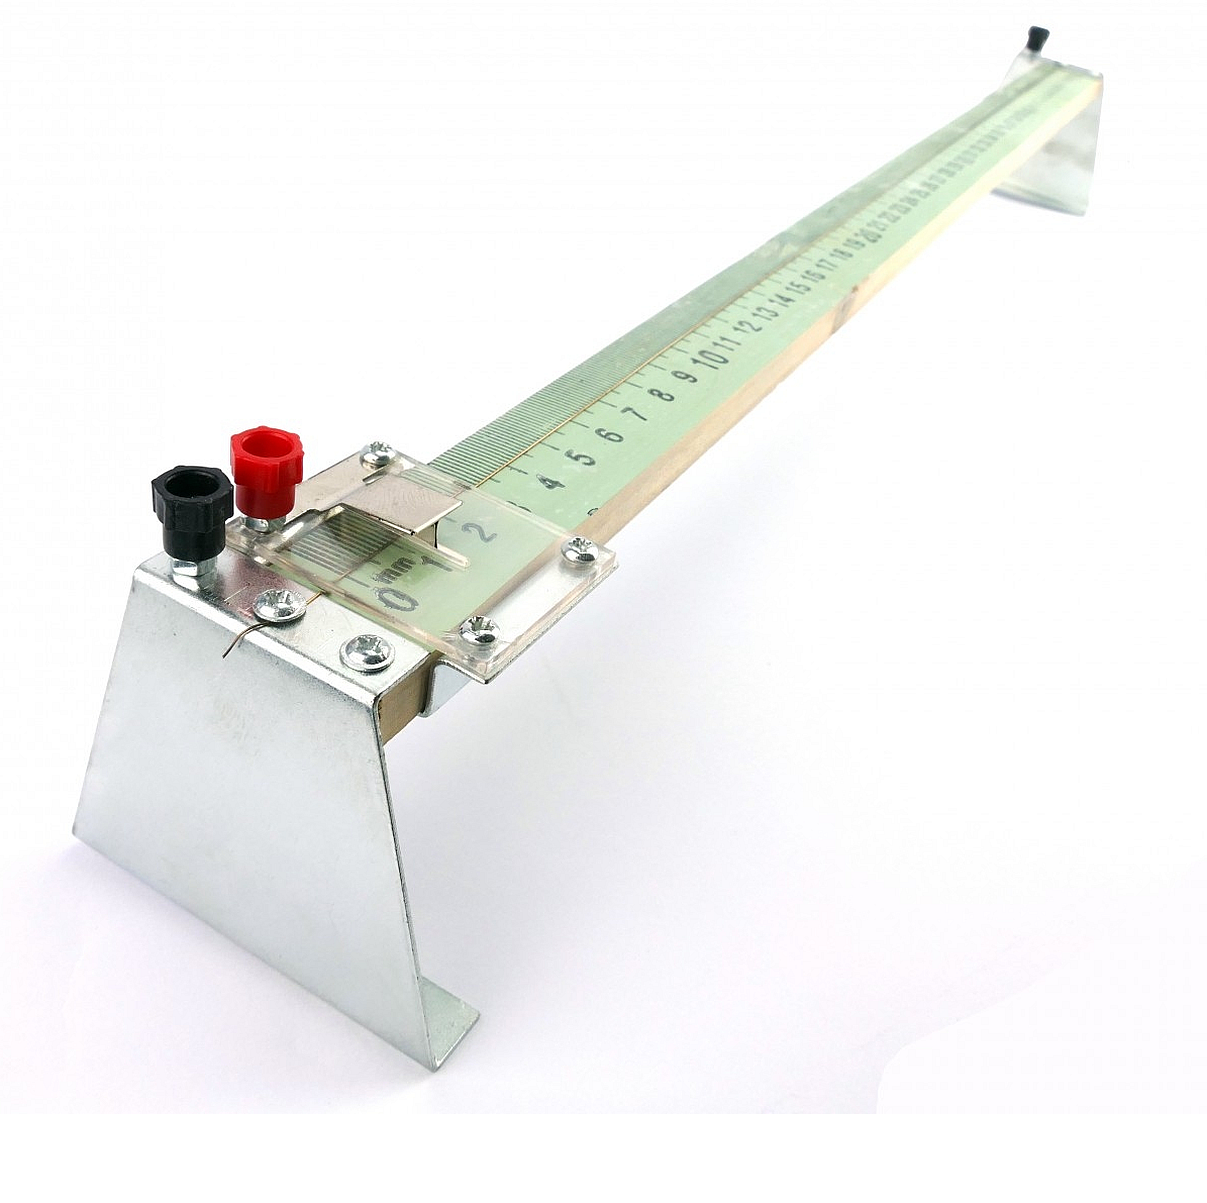
\includegraphics[width=1\linewidth]{reochord}
%		\caption{Реохорд}
%		\label{pic:reochord}
%\end{tornpage}
%\end{minipage}
%\quad%---------------------------------------------------------
%\begin{minipage}[t]{0.47\linewidth}
%\begin{tornpage}\centering
%		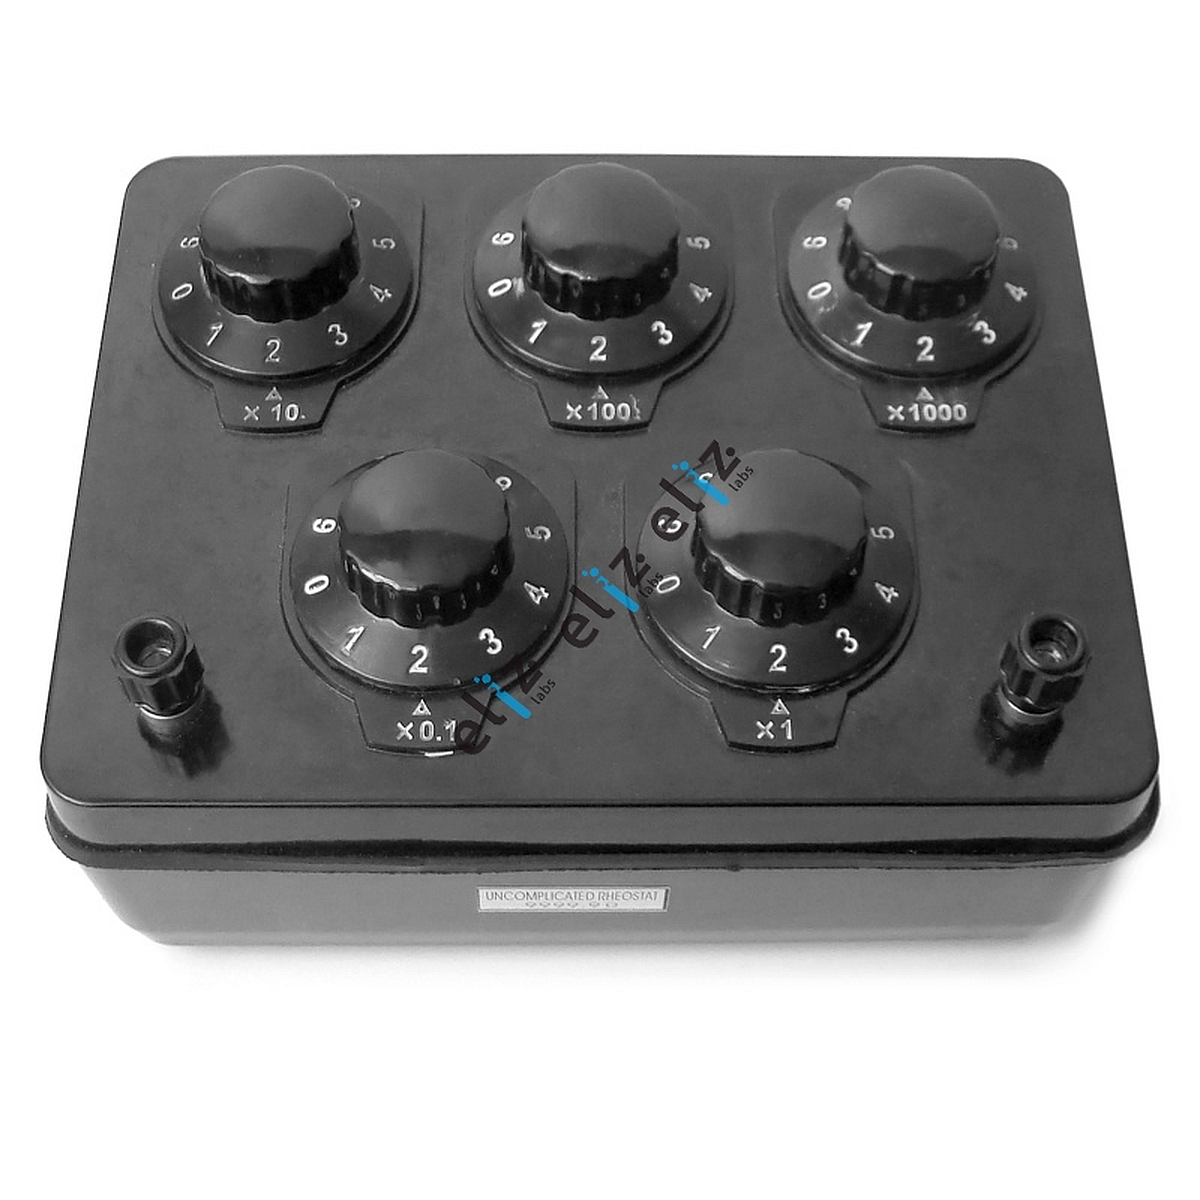
\includegraphics[width=1\linewidth]{Rmag}
%		\caption{Магазин опорів}
%		\label{pic:reochord}
%\end{tornpage}
%\vspace*{10pt}
%\end{minipage}
%\begin{minipage}[t]{0.47\linewidth}
%\begin{tornpage}\centering
%		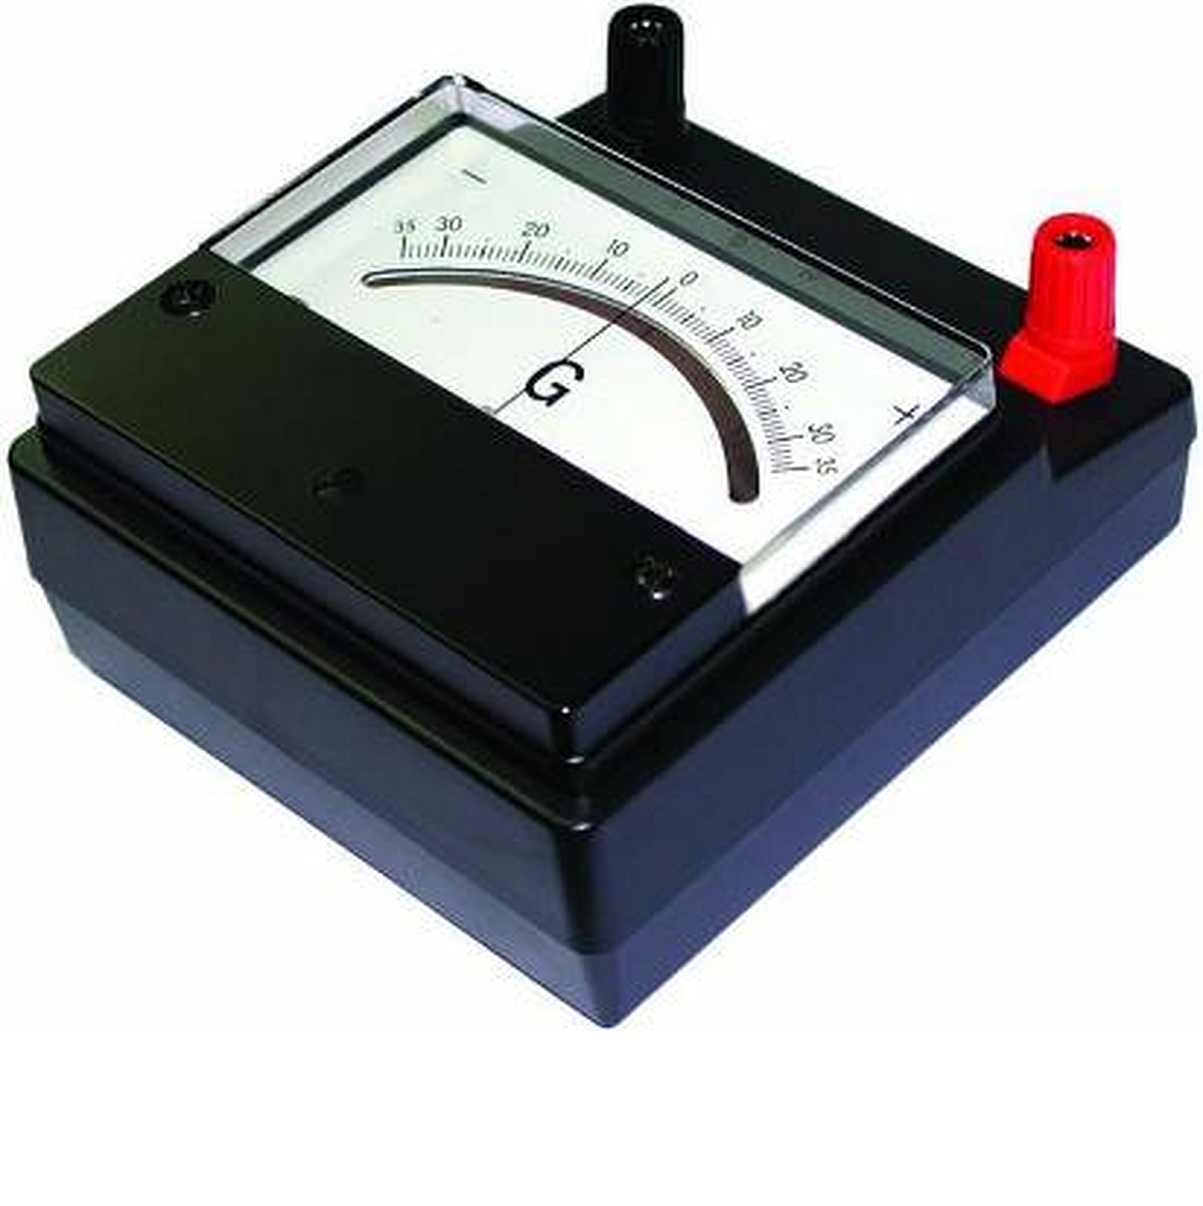
\includegraphics[width=1\linewidth]{galvanometer}
%		\caption{Гальванометр}
%		\label{pic:galvanometer}
%\end{tornpage}
%\end{minipage}
%\quad%---------------------------------------------------------
%\begin{minipage}[t]{0.47\linewidth}
%\begin{tornpage}\centering
%		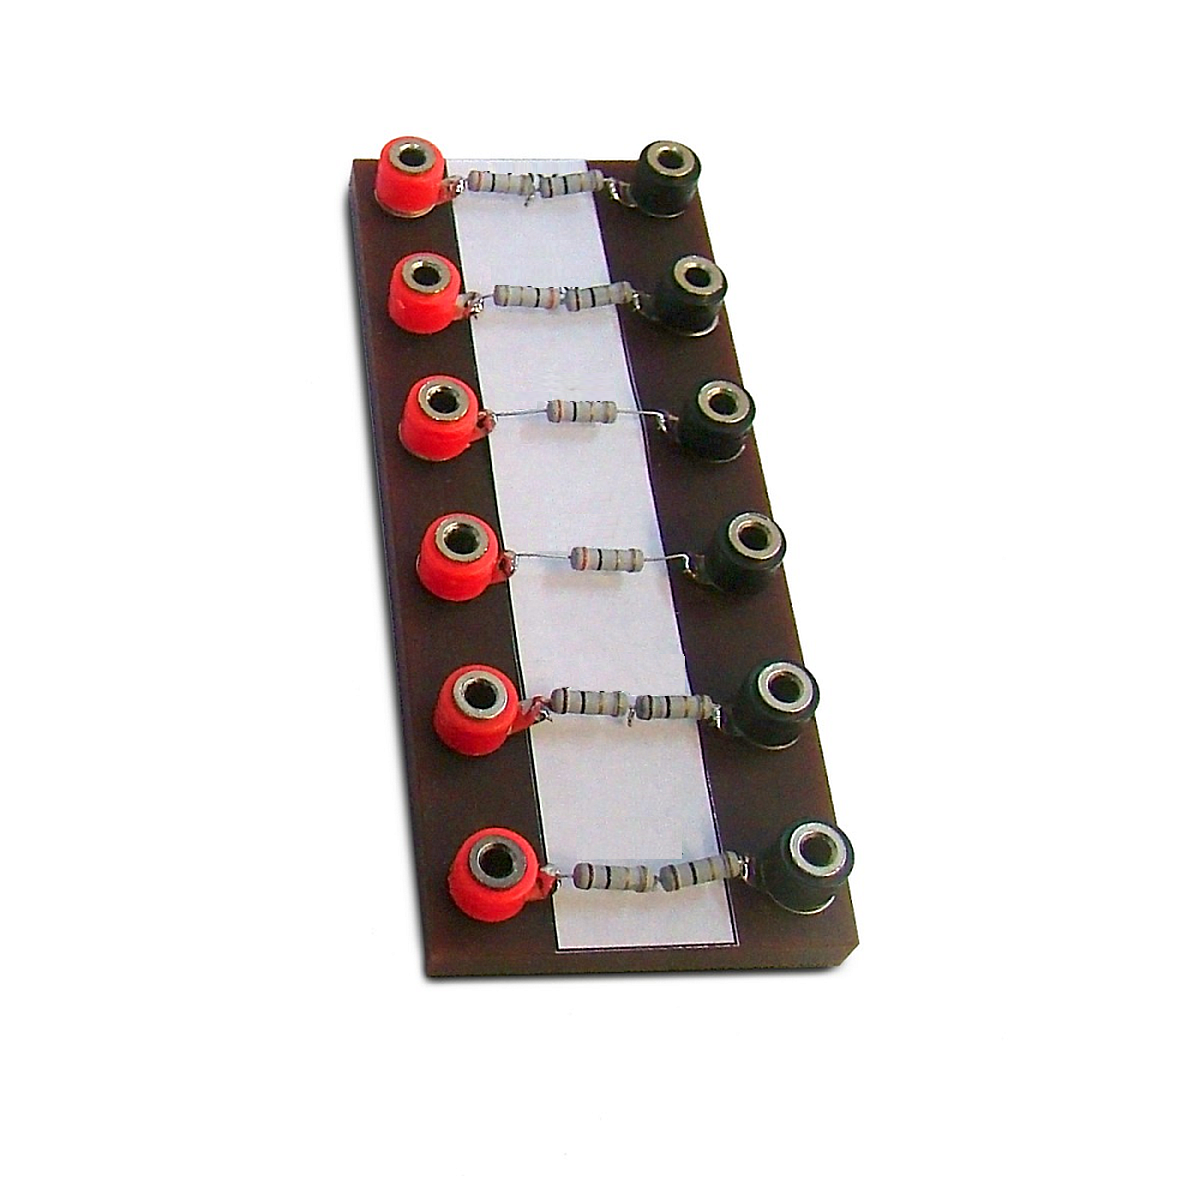
\includegraphics[width=1\linewidth]{resistors}
%		\caption{Резистори}
%		\label{pic:resistors}
%\end{tornpage}
%\end{minipage}
%%---------------------------------------------------------
%\end{figure}
%%=========================================================



\section{Хід експерименту}

\begin{enumerate}
	\item Зібрати схему, зображену на рис.~\ref{MeasurBridge}.
	\item Повзунок поставте точно посередині реохорда. \label{item2}
	      \begin{itemize}
		      \item На магазині опорів всі декади встановіть на нульові поділки.
		      \item  Натисніть кнопку на короткий час ($1 - 2$ секунди) і запам'ятайте, в який бік відхилилася стрілка гальванометра.
                \begin{More}
                
		            Кнопку не слід тримати натиснутою довго, щоб реохорд і резистори не встигали сильно нагрітися, інакше ускладнюється процес врівноваження моста.
                
                \end{More}


		      \item Встановіть на магазині опір $R$ близьким $10\ 000$~Ом. Знову натисніть кнопку і зверніть увагу, в який бік
		            відхилилася стрілка гальванометра в цьому випадку. Якщо вона відхилилася в протилежну сторону в порівнянні з першим виміром при нульовому опорі, то шукана величина знаходиться між цими межами. Необхідно знайти її в грубому наближенні, обертаючи ручки старших декад магазину до тих пір, поки стрілка гальванометра буде відхилятися від нуля на $2-3$ поділки.
		      \item Після цього вже молодшими декадами магазину $R$ доможіться найкращого балансування містка, коли при натисканні кнопки стрілка гальванометра залишається на місці.
		      \item Запишіть відлік на магазині опорів $R$, при яку досягнуто рівновагу містка.
		      \item Розрахуйте значення $R_x$.
	      \end{itemize}
	\item Змістіть повзунок реохорда вліво на $10 \ldots 20$~мм, запишіть довжини плечей при новому положенні повзунка. Проведіть всі операції врівноваження моста, як це сказано вище, в п.~\ref{item2}.

	      Повторіть так кілька разів. Таким чином, у вас вийде кілька вимірів опору одного і того ж резистора $R_x$.
	\item Замініть $R_x$ і виміряйте його опір.
	\item З'єднайте опори послідовно і виміряйте їх опір.
	\item З'єднайте опори паралельно і виміряйте їх опір.
	\item Величини загальних опорів при послідовному і паралельному з'єднанні, знайдені шляхом вимірювань, порівняйте з відповідними величинами опорів, отриманими в результаті розрахунку за формулами паралельного і послідовного з'єднання провідників.
\end{enumerate}

\section{Контрольні питання}

\begin{enumerate}
	\item Сформулюйте закон Ома для однорідної та неоднорідної ділянки кола.
	\item Від яких величин залежить опір ізотропного провідника?
	\item Сформулюйте закони Кірхгофа, поясніть їх застосування.
	\item Використовуючи закони Кірхгофа, виведіть умови рівноваги містка Уітстона.
	\item Чи зміниться умова рівноваги моста, якщо гальванометр і джерело струму поміняти місцями?
	\item Чому гальванометр, застосовуваний в мосту Уітстона, має двосторонню шкалу з нулем посередині?
	\item Оцініть похибка методу. За якої умови похибка методу буде мінімальною?
    \item Які способи вимірювання електричного опору існують? Які переваги і недоліки вони мають в порівнянні з містковою схемою і один з одним?
\end{enumerate}

\end{document}
